\chapter{Primal Formulation with Non-Linear Model}\label{chap: deep}

In Chapter~\ref{chap: framework} we introduced general framework for binary classification at the top samples, and showed multiple formulations that fall into it. All these formulations are summarized in Table~\ref{tab: summary formulations}. In Chapter~\ref{chap: linear}, we discussed theoretical properties of all formulations for special case of linear model. Since many real world problems are not lineary separable, in Chpater~\ref{chap: dual}, we derived dual forms of all formulations and emply non-linear kernels. Moreover, we derived efficient algorithm to solve these dual formulations. Even though we derived a way how to use non-linear model, the dual formulations are not suitable for large data. For this reason, in this chapter, we focus on the case, when the general model~$f$ is used. we focus only on formulations that use surrogate false-negative rate as an objective function, i.e. we have the following formulation
\begin{mini}{\bm{w}, \, t}{
  \frac{1}{2} \norm{\bm{w}}^2 + \frac{1}{\npos} \fns(\bm{s}, t)
  }{\label{eq: aatp deep general}}{}
  \addConstraint{s_i}{= f(\bm{x}_i; \bm{w}), \quad i \in \I}
  \addConstraint{t}{= G\Brac{\bm{s}, \bm{y}},}
\end{mini}
where~$f$ is an arbitrary model. 


Our goal is to derive method how to solve formulations from Table~\ref{tab: summary formulations} for large data. The standard way is to use stochastic gradient descent. To do so, we need to know the gradient of the objective function. For this reason, the whole section assumes that the classifier~$f$ is differentiable. The optimization problem~\eqref{eq: aatp deep general} depends on two decision variables~$\bm{w}$ and~$t.$ However, for all formulations from Table~\ref{tab: summary formulations} and for each~$\bm{w}$, the threshold~$t$ can be computed uniquely. We stress this dependence by writing~$t(\bm{w})$ instead of~$t$. By doing so, we effectively remove the threshold~$t$ from the decision variables and~$\bm{w}$ remains the only decision variable. Denoting the objective of~\eqref{eq: aatp deep general} by~$L(\bm{w})$
\begin{equation*}
  L(\bm{w})
    = \frac{1}{2}\norm{\bm{w}}^2 + \frac{1}{\npos} \sum_{i \in \Ipos} l \Brac{t(\bm{w}) - f(\bm{x}_i; \bm{w})},
\end{equation*}
the chain rule implies that the gradient is equal to
\begin{equation}\label{eq: deep L gradient true}
  \nabla L(\bm{w})
    = \bm{w} + \frac{1}{\npos} \sum_{i \in \Ipos} l'\Brac{t(\bm{w}) - f(\bm{x}_i; \bm{w})}\Brac{\nabla t(\bm{w}) - \nabla f(\bm{x}_i; \bm{w})}.
\end{equation}
The only remaining part is the computation of~$\nabla t(\bm{w})$. It is simple for most of the formulations from Table~\ref{tab: summary formulations}. Moreover, Theorem~\ref{thm: differentiability} shows the computation for \PatMat.

The basic idea of the stochastic gradient descent is to split the dataset into several small minibatches~$\Imb^1, \, \Imb^2, \ldots, \, \Imb^m$ and at each iteration perform all operations on one minibatch. For standard problems it can be performed seamlessly, since these problems are decomposable. However, in our case, the decision threshold~$t$ depends \emph{all} scores~$\bm{s}.$ Therefore, the objective is non-additive and non-decomposable due to the threshold. To apply the stochastic gradient descent, we need to use some approximation the true threshold. The most straightforward way is to use the same rule as for the whole dataset and compute the samplesd threshold~$\hat{t}$ only on data from the minibatch. By replacing the sum over all positive samples~$\Ipos$ with a sum over all positive samples in a minibatch~$\Imbpos,$ and the true threshold~$t$ by its samples version~$\hat{t},$ ew get the approximation of the true gradient 
\begin{equation}\label{eq: deep L gradient sampled}
  \nabla \hat{L}(\bm{w})
    = \bm{w} + \frac{1}{\nmbpos} \sum_{i \in \Imbpos} l'\Brac{\hat{t}(\bm{w}) - f(\bm{x}_i; \bm{w})}\Brac{\nabla \hat{t}(\bm{w}) - \nabla f(\bm{x}_i; \bm{w})}.
\end{equation}
where~$\nmbpos$ denotes the number of positive samples in the minibatch. Using the sampled gradient above, the whole procedure of stochastic gradient descent for formulations from Table~\ref{tab: summary formulations} is summarized in Algorithm~\ref{alg: deep basic}.

\begin{algorithm}
  \centering
  \begin{algorithmic}[1]
    \Require Dataset~$\mathcal{D}$, minibatches~$\Imb^1,\; \Imb^2, \ldots, \; \Imb^m$, and stepsize~$\alpha^k$
    \State Initialize weights~$\bm{w}^0,$ $k \gets 0$
    \Repeat
    \State Select a minibatch~$\Imb^k$
    \State Compute scores~$s_i \gets f(\bm{x}_i; \bm{w})$ for all~$i \in \Imb^k$
    \State Compute samples thershold~$\hat{t} \gets G(\bm{s}_{\text{mb}}, \bm{y}_{\text{mb}})$
    \State Compute sampled gradient~$\nabla \hat{L}$ based on~$\Imb^k$ according to~\eqref{eq: deep L gradient sampled}
    \State Set~$\bm{w}^{k+1} \gets \bm{w}^k - \alpha^k \cdot \nabla \hat{L}$
    \State Set~$k \gets k + 1$
    \Until{stopping criterion is satisfied}
  \end{algorithmic}
  \caption{Basic algorithm for solving~\eqref{eq: aatp deep general}}
  \label{alg: deep basic}
\end{algorithm}

\section{Bias of Sampled Gradient}

In the previous section, we derived general procedure for stochastic gradient descent that can be used for any formulation from Table~\ref{tab: summary formulations} that uses surrogate false-negative rate as an objective function. The problem of this procedure is, that the sampled threshold~$\hat{t}$ is computed only from data from one minibatch using the same formula as for the whole dataset. However, such a choice of sampled threshold~$\hat{t}$ underestimates the true value. This is especially evident for \TopPush, where the sampled maximum is always smaller or equal to the true maximum. Therefore, the sampled threshold is a biased estimate of the true threshold. Figure~\ref{fig:thresholds1} illustrates this phenomenon. The bias between the true and sampled thresholds is large even for medium-sized minibatches. Backpropagation then propagates this sampling error through the whole gradient, and consequently, the minibatch gradient is a biased estimate of the true gradient. This brings numerical issues~\cite{bottou2018optimization}.

\begin{figure}
  \centering
  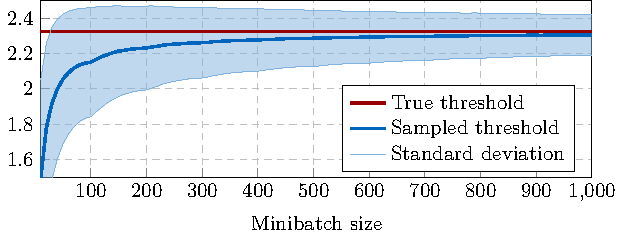
\includegraphics[width = \linewidth]{images/deep_threshold_bias.pdf}
  \caption{The bias between the sampled and true thresholds computed from scores following the standard normal distribution. The threshold separates the top~$1\%$ of samples with the highest scores.}
  \label{fig:thresholds1}
\end{figure}

Convergence proofs of the stochastic gradient descent require that the sampled gradient is an unbiased estimate of the true gradient~\cite{bottou2018optimization}. This means that
\begin{equation}\label{eq:defin_bias}
  \bias(\bm{w}) := \nabla L(\bm{w}) - \EE \nabla \hat{L}(\bm{w})
\end{equation}
equals to~$0$ for all~$\bm{w}$. A comparison of \eqref{eq: deep L gradient true} and \eqref{eq: deep L gradient sampled} shows that a necessary condition is that the sampled threshold~$\hat{t}$ is an unbiased estimate of the true threshold~$t$. However, as we discussed above, it is not a case for Algorithm~\ref{alg: deep basic}. The next proposition quantifies the difference between the sampled and true thresholds for methods that use quantile as threshold.

\pagebreak

\begin{proposition}[\cite{glynn1996importance}]\label{proposition:bound}
  Consider an absolutely continuous random variable~$X$ with distribution function~$F.$ Let $X_1,\, X_2, \ldots, \, X_n$ be i.i.d. samples from~$X$ and let~$\tau \in (0,1).$ Denote the true quantile~$t$ and its sampled version as~$\hat{t}$
  \begin{align*}
    t & = F^{-1}(1 - \tau), &
    \hat{t} & = F_{n}^{-1}(1 - \tau), &
  \end{align*}
  where~$F_{n}$ is the empirical distribution function. If~$F$ is differentiable with a positive gradient at~$t$, then
  \begin{equation*}
    \sqrt{n}\Brac{t - \hat{t}} \rightarrow \mathcal{N} \Brac{0, \; \frac{\tau(1-\tau)}{F'(t)^2}},
  \end{equation*}
  where the convergence is in distribution and~$\mathcal{N}$ denotes the normal distribution.
\end{proposition}

This proposition states that when the minibatch size increases to infinity, the variance of the sampled threshold is approximately
\begin{equation*}
  \frac{\tau(1-\tau)}{nF'(t)^2}.
\end{equation*}
Figure~\ref{fig:thresholds1} shows this empirically for the case where the scores follow the standard normal distribution and~$\tau=0.01$ is the desired top fraction of all samples. The approximation is poor with both large bias and standard deviation. The natural choice to mitigate the bias is to work with large minibatches. Even though this is not a standard way, some works suggest this route~\cite{you2019large}. When the minibatch is large, it contains more samples and the sampled threshold is more precise. This approach is applicable to any method from Table~\ref{tab: summary formulations}.

\section{\DeepTopPush}

In the previous sections we derived Algorithm~\ref{alg: deep basic} that can be used for any formulation from Table~\ref{tab: summary formulations} that uses surrogate false-negative rate as an objective function. However, this approach provides biased gradient and the only way how to reduce the biass is to use large minibatches. In this section, we derive new method \DeepTopPush, that mitigates this bias in different way.

We start with \TopPush formulation presented in~\cite{li2014top}. Authors of~\cite{li2014top} proposed the \TopPush formulation with linear model and solved it in its dual form. In Section~\ref{sec: ranking} we generalized this formulation for general model~$f,$ and in Chapter~\ref{chap: linear} we solved the formulation directly in its primal form for linear classifiers. For general model~$f,$ we stay in the primal form to be able to employ stochastic gradient descent. It means that we have the following optimization problem
\begin{mini}{\bm{w}, \, t}{
  \frac{1}{\npos} \fn(\bm{s}, t)
  }{\label{eq: toppush deep}}{}
  \addConstraint{s_i}{= f(\bm{x}_i; \bm{w}), \quad i \in \I}
  \addConstraint{t}{= \max_{j \in \Ineg} \; s_{j}.}
\end{mini}
Since the threshold always equals to one of the scores~\cite{boyd2012accuracy}, its computation has a simple local formula. In other words, if the highest negative score corresponds to sample~$\bm{x}_{\indmax},$ then the gradient of the threshold equals
\begin{equation*}
  \nabla t = f(\bm{x}_{\indmax}; \bm{w}).
\end{equation*}
Therefore, the gradient of the objective function of~\eqref{eq: toppush deep} reads
\begin{equation}\label{eq: deep L gradient true toppush}
  \hat{L}(\bm{w})
    = \bm{w} + \frac{1}{\npos} \sum_{i \in \Ipos} l'\Brac{f(\bm{x}_{\indmax}; \bm{w}) - f(\bm{x}_i; \bm{w})}\Brac{\nabla f(\bm{x}_{\indmax}; \bm{w}) - \nabla f(\bm{x}_i; \bm{w})}.
\end{equation}
Then , using the same transition to the minibatches as in previous section, we get the formula for sampled gradient
\begin{equation}\label{eq: deep L gradient sampled toppush}
  \hat{L}(\bm{w})
    = \bm{w} + \frac{1}{\nmbpos} \sum_{i \in \Imbpos} l'\Brac{f(\bm{x}_{\indmaxmb}; \bm{w}) - f(\bm{x}_i; \bm{w})}\Brac{\nabla f(\bm{x}_{\indmaxmb}; \bm{w}) - \nabla f(\bm{x}_i; \bm{w})},
\end{equation}
where~$\indmaxmb$ represents the index of the negative sample with highest score from the minibatch. As discussed before, such a choice of the decision threshold provides a lower estimate of the true threshold. To improve this approximation, we modify the idea presented in~\cite{adam2019machine}. When the weights~$\bm{w}$ of model~$f$ are updated using stochastic gradient descent, the scores~$\bm{s}$ usually do not change much. It is true especially for a small learning rates. This means that if a sample has the highest score, it will likely have the highest score even after the gradient step. Since the threshold~$t$ for \TopPush equals the highest score corresponding to negative samples, we can easily track to which sample this score corresponds. Therefore, we can enhance the current minibatch by the sample that represents the treshold in the previous minibatch. This significantly increases the chance that the sampled threshold equals the true threshold. The whole procedure is summarized in Algorithm~\ref{alg: deep toppush}.

\begin{algorithm}[H]
  \centering
  \begin{algorithmic}[1]
    \Require Dataset~$\mathcal{D}$, minibatches~$\Imb^1,\; \Imb^2, \ldots, \; \Imb^m$, and stepsize~$\alpha^k$
    \State Initialize weights~$\bm{w}^0,$ $k \gets 0,$ and random index~$\indmaxmb$
    \Repeat
    \State Select a minibatch~$\Imb^k$
    \State Enhance minibatch~$\Imb^{\text{enh}} = \Imb^k \cup \Brac[c]{\indmaxmb}$
    \State Compute scores~$s_i \gets f(\bm{x}_i; \bm{w})$ for all~$i \in \Imb^{\text{enh}}$
    \State Find index of sampled thershold~$\indmaxmb \gets \argmax \Set{s_j}{j \in \Imb^{\text{enh}} \cap \Ineg}$
    \State Compute sampled gradient~$\nabla \hat{L}$ based on~$\Imb^{\text{enh}}$ according to~\eqref{eq: deep L gradient sampled toppush}
    \State Set~$\bm{w}^{k+1} \gets \bm{w}^k - \alpha^k \cdot \nabla \hat{L}$
    \State Set~$k \gets k + 1$
    \Until{stopping criterion is satisfied}
  \end{algorithmic}
  \caption{\DeepTopPush as an efficient method for maximizing accuracy at the top.}
  \label{alg: deep toppush}
\end{algorithm}

\begin{note}[Other formulations]\label{note: deep extension}
  Algorithm~\ref{alg: deep toppush} is applicable only on the \TopPush formulation, since all other formulations uses more samples to compute the threshold. However, we can modify the algortihm to be usable for example with \TopPushK formulation. Since \TopPushK uses hte mean of~$K$ highest negative scores as a threshold, we need to enhance the minibatch by~$K$ indices that corresponds to the $K$ highest negative scores. However, since our goal was to use small minibatches, such an approach is trackatble only for small~$K.$ 
\end{note}

\section{Theoretical justification}

Even though this result gives us insight into the bias of the sampled threshold, we are ultimately interested in the bias of the sampled gradient~$\nabla \hat{L}(\bm{w})$. To do so, recall that~$\indmax$ is index of true threshold on the whole dataset, while~$\indmaxmb$ is the index of sampled threshold on the minibatch. We split the computation based on whether these two indices are identical or not.

\begin{restatable}{lemma}{lemmacovergencedeep}\label{lemma:convergence}
  Let~$\indmax$ be unique. Assume that the selection of positive and negative samples into the minibatch is independent and that the threshold is computed from negative samples while the objective is computed from positive samples. Then the conditional expectation of the sampled gradient satisfies
  \begin{equation*}
    \EE\Brac[s]{\nabla \hat{L}(\bm{w}) \middle\vert\indmaxmb=\indmax} =  \nabla L(\bm{w}).
  \end{equation*}
\end{restatable}

\begin{restatable}{theorem}{thmcovergencedeep}\label{theorem:convergence}
  Under the assumptions of Lemma~\ref{lemma:convergence}, the bias of the sampled gradient from \eqref{eq:defin_bias} satisfies
  \begin{equation}\label{eq:comp_bias}
    \bias(\bm{w}) = \PP\Brac[s]{\indmaxmb\neq \indmax} \Brac{\nabla L(\bm{w}) - \EE\Brac[s]{\nabla \hat{L}(\bm{w}) \middle\vert \indmaxmb\neq \indmax}}.
  \end{equation}
\end{restatable}

The assumptions of Theorem~\ref{theorem:convergence} holds only for \TopPush, but it can be extended for other formulations as discussed in Note~\ref{note: deep extension}. The bias \eqref{eq:comp_bias} consists of a multiplication of two terms. As we discussed in the previous sections, there are two strategies to reduce the bias:
\begin{enumerate}
  \item \textbf{Large minibatches:} When the minibatch is large, it contains more samples and the chance that~$\indmaxmb$ differs from~$\indmax$ decreases. This reduces the first term in~\eqref{eq:comp_bias}. Moreover, Proposition~\ref{proposition:bound} ensures that the difference between the sampled threshold~$\hat{t}$ and the true threshold~$t$ is small. Then the difference between the true gradient~\eqref{eq: deep L gradient true toppush}and the sampled gradient~\eqref{eq: deep L gradient sampled toppush} decreases as well. This reduces the second term in~\eqref{eq:comp_bias}.
  \item \textbf{Enhanced minibatch:} The enhanced minibatch increase the chance that~$\indmaxmb$ equals~$\indmax.$ This reduces the first term in~\eqref{eq:comp_bias}. 
\end{enumerate}
The former strategy uses Algorithm~\ref{alg: deep basic} while the later strategy is described only for formulation~\eqref{eq: toppush deep} in Algorithm~\ref{alg: deep toppush}. For clarity in the following text, we use name \DeepTopPush for procedue that solves formulation~\eqref{eq: toppush deep} using Algorithm~\ref{alg: deep toppush}. Moreover, we use name \TopPush for procedue that solves formulation~\eqref{eq: toppush deep} using Algorithm~\ref{alg: deep basic}

Figure~\ref{fig:thresholds2} the effect of the enhanced minibatch to the training. The top part of the figure compares the value of the true threshold~$t$ and its sampled version~$\hat{t}$ during training (\textbf{top}). The red dashed line represents true threshold~$t.$ The full blue line shows the behaviour of \DeepTopPush (enhanced minibatch) and the dotted grey dotted line shows \TopPush. While the sampled threshold for \TopPush jumps wildly, the sampled threshold for \DeepTopPush is smooth and often equals the true threshold. It shows the importance of the enhanced minibatch. Moreover, Theorem~\ref{theorem:convergence} then implies that for \DeepTopPush the sampled gradient is an unbiased estimate of the true gradient. This is even more pronounced in the bottom part of Figure~\ref{fig:thresholds2}, which shows the angle between the true gradient~$\nabla L$ and the sampled gradient~$\nabla \hat{L}.$ This angle is important because~\cite{nocedal2006numerical} showed that if this angle is uniformly in the interval~$[0, 90)$, then gradient descent schemes converge. This is precisely what happened for \DeepTopPush. When the threshold is correct, the true and estimated gradients are parallel to each other, and the gradient descent moves in the correct direction.

\begin{figure}
  \centering
  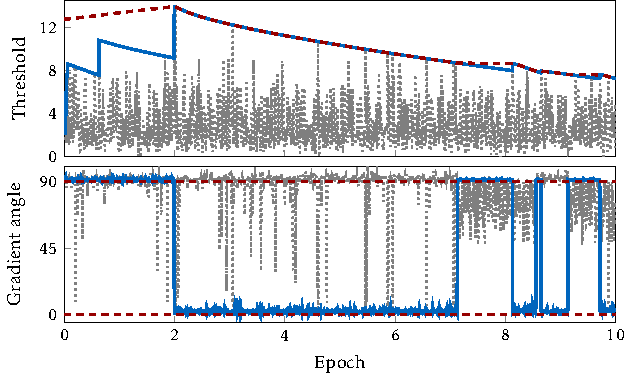
\includegraphics{images/deep_thresholds.pdf}
  \caption{The thresholds (\textbf{top}) and angle between true and sampled gradients (\textbf{bottom}) for \DeepTopPush using Algorithm~\ref{alg: deep toppush} (full blue line) and \TopPush using Algorithm~\ref{alg: deep basic} (dotted gray). The experiment was performed on CIFAR10 dataset with minibatch size 32 and 10 training epochs.}
  \label{fig:thresholds2}
\end{figure}